\documentclass[border=4pt]{standalone}
\usepackage{amsmath,amssymb}
\usepackage{tikz}
\begin{document}
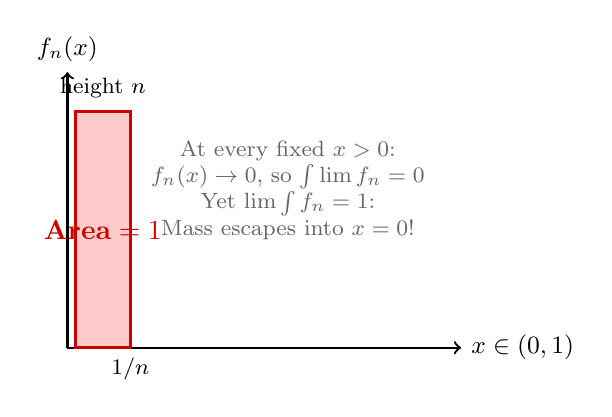
\begin{tikzpicture}[font=\small]
  \draw[->, thick] (0,0) -- (5.0,0) node[right] {$x \in (0,1)$};
  \draw[->, thick] (0,0) -- (0,3.5) node[above] {$f_n(x)$};

  % Spike
  \draw[very thick, fill=red!20, draw=red!80!black] (0.1, 0) rectangle (0.8, 3.0);
  \node[red!80!black, font=\bfseries] at (0.45, 1.5) {$\text{Area} = 1$};
  \node[font=\footnotesize] at (0.45, 3.3) {height $n$};
  \node[below, font=\footnotesize] at (0.8, 0) {$1/n$};

  \node[font=\footnotesize, text=gray!80!black, align=center] at (2.8, 2.0) 
    {At every fixed $x > 0$:\\$f_n(x) \to 0$, so $\int \lim f_n = 0$\\Yet $\lim \int f_n = 1$:\\Mass escapes into $x=0$!};
\end{tikzpicture}
\end{document}